\documentclass[11pt, a4paper]{article}

% --- Packages ---
\usepackage[utf8]{inputenc} % Encoding
\usepackage{amsmath, amssymb, amsthm} % Advanced math typesetting
\usepackage{physics} % Useful commands for physics (derivatives, vectors, braket)
\usepackage{graphicx} % For including diagrams and images
\usepackage{geometry} % Page margins
\usepackage{siunitx} % For proper formatting of SI units
\usepackage{fancyhdr} % Custom headers and footers
\usepackage{xcolor} % For blocks of color
\usepackage{enumitem} % For enumerated lists with letters
\usepackage{float} % For figure strict positioning
\usepackage{parskip} % Elimina la sangría y añade espacio entre párrafos

% --- Page Setup ---
\geometry{top=2.5cm, bottom=2.5cm, left=2.5cm, right=2.5cm}
\pagestyle{fancy}
\fancyhf{} % Clear all default header and footer fields
\fancyhead[L]{\textbf{José Carlos López Henestrosa}}
\fancyhead[R]{Fundamentos físicos de la informática - PEC1}
\fancyfoot[C]{\thepage} % Page number at the bottom center

% --- Custom Environments ---
% Creates a neat "Problem X" environment
% --- Custom Environments ---
\newenvironment{problem}[1][Cuestión]{
		\vspace{0.5cm}
		\noindent{\Large\bfseries #1} \par\vspace{0.5cm}
}{
		\vspace{0.5cm}
}

% --- Document Starts Here ---
\begin{document}
	% --- Title Block ---
	\begin{center}
		\Large{ \textbf{PEC1} } \\
		\vspace{0.5cm}
		\normalsize{\textbf{Nombre:} José Carlos López Henestrosa} \\
		\vspace{0.5cm}
		\normalsize{Declaro que ostento la autoría total y llena de todas las tareas que se llevan a cabo en el presente documento. Soy la única persona que ha elaborado cada ejercicio. No he compartido los enunciados con nadie y la única ayuda que he recibido ha sido a través del aula de la UOC y su profesorado y he citado de forma explícita los recursos externos que he usado en la preparación de la PEC.} \\
		\vspace{0.5cm}
		\normalsize{Todas las referencias académicas en esta entrega hacen referencia a los libros \textit{Circuitos eléctricos} y \textit{Circuitos RLC} de los recursos de esta asignatura, salvo que se cite otra fuente explícitamente.}
	\end{center}

	\vspace{1cm}
	\hrule
	\vspace{1cm}

	% --- Exercise 1 ---
	\begin{problem}[Cuestión 1]
		Tenemos el circuito de la figura 1:

		\begin{figure}[H]
			\centering
			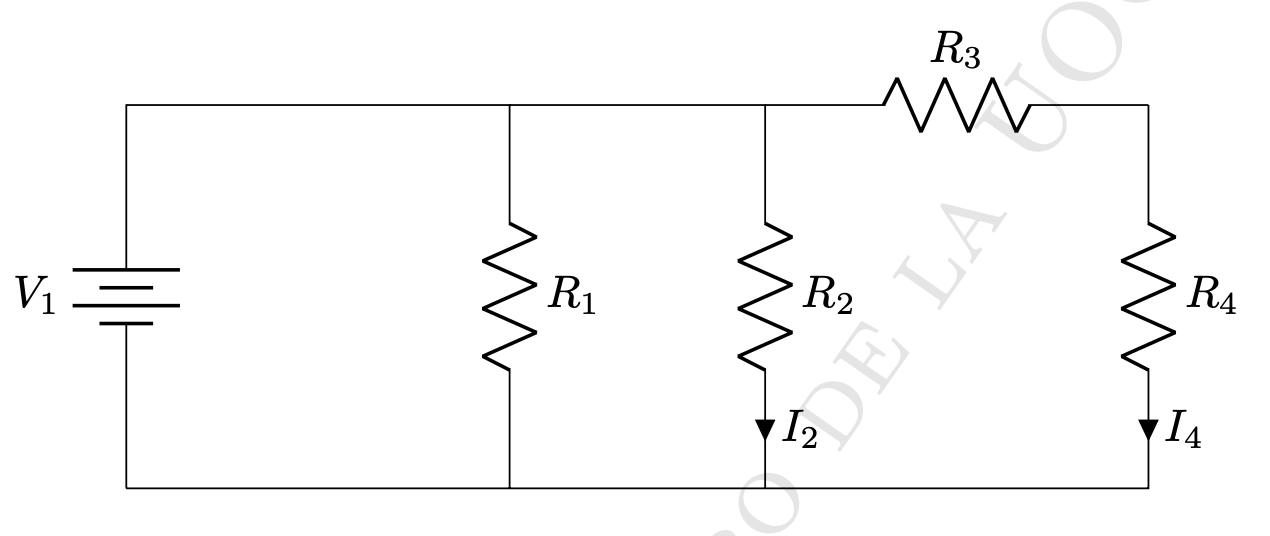
\includegraphics[width=10cm]{imagenes/enunciados/1_enunciado.png}
			\caption{Circuito de la Cuestión 1.}
		\end{figure} 

		donde $V_1=10 \text{ V}, I_2=0,5 \text{ A}, R_1=75 \; \Omega, R_3 = 20 \; \Omega \text{ y } R_4=30 \; \Omega$

		{ \color{blue} 
			\textbf{NOTA:} Todas las fórmulas de esta cuestión han sido tomadas del libro \textit{Circuitos eléctricos}.
		}

		\begin{enumerate}[label=\alph*)] 
			\item Determinar el valor de la resistencia $R_2$.

				{ \color{blue} 
					Dado que los componentes del circuito se encuentran en una asociación en paralelo, la diferencia de potencial es la misma para los extremos de todas las ramas. Por lo tanto, la tensión aplicada a la resistencia $R_2$ es exactamente la tensión de la fuente, es decir, $V_1 = 10 \text{ V}$.

					Conociendo la tensión y la intensidad que circula por la rama ($I_2 = 0,5 \text{ A}$), podemos calcular la resistencia aislando su valor de la ley de Ohm. Utilizando la ecuación (9) del libro:
					$$R_2 = \frac{V_1}{I_2}$$

					Sustituyendo los valores proporcionados:
					$$\boxed{R_2 = \frac{10 \text{ V}}{0,5 \text{ A}} = 20 \; \Omega}$$
				}

			\vspace{0.5cm}

			\item Determinar el valor de la corriente $I_4$.

				{ \color{blue} 
					La corriente $I_4$ circula a través de la rama formada por las resistencias $R_3$ y $R_4$. Al estar estas dos colocadas en serie, podemos calcular la resistencia equivalente de esta rama mediante la suma de sus valores individuales, según se define en la ecuación (14):

					$$R_{34} = R_3 + R_4 = 20 \; \Omega + 30 \; \Omega = 50 \; \Omega$$

					Esta rama equivalente ($R_{34}$) se encuentra en paralelo con la fuente principal, por lo que la caída de tensión en todo el conjunto es de nuevo $V_1 = 10 \text{ V}$. 

					Para hallar la corriente $I_4$, aplicamos la ley de Ohm descrita en la ecuación (5) del libro:
					$$I_4 = \frac{V_1}{R_{34}}$$

					Sustituyendo los valores:
					$$\boxed{I_4 = \frac{10 \text{ V}}{50 \; \Omega} = 0,2 \text{ A}}$$
				}

			\item Determinar el valor de la resistencia equivalente del circuito.

				{ \color{blue} 
					Para calcularlo, nos fijamos en que el sistema está compuesto por tres ramas principales dispuestas en paralelo:
					\begin{itemize}
						\item Rama 1: $R_1 = 75 \; \Omega$
						\item Rama 2: $R_2 = 20 \; \Omega$ (calculada en el apartado a)
						\item Rama 3: $R_{34} = 50 \; \Omega$ (calculada en el apartado b)
					\end{itemize}

					En el caso general para varias resistencias colocadas en paralelo, la resistencia equivalente se calcula como el inverso de la suma de los inversos de las resistencias originales, como indica la ecuación (24):
					$$\frac{1}{R_{eq}} = \frac{1}{R_1} + \frac{1}{R_2} + \frac{1}{R_{34}}$$

					Sustituyendo los valores calculados:
					$$\frac{1}{R_{eq}} = \frac{1}{75} + \frac{1}{20} + \frac{1}{50}$$

					Hallamos un denominador común (300) para realizar la suma:
					$$\frac{1}{R_{eq}} = \frac{4}{300} + \frac{15}{300} + \frac{6}{300} = \frac{25}{300} = \frac{1}{12} \; \Omega^{-1}$$

					Despejamos finalmente $R_{eq}$:
					$$\boxed{R_{eq} = 12 \; \Omega}$$
				}
		\end{enumerate}
	\end{problem}

	% --- Exercise 2 ---
	\begin{problem}[Cuestión 2]
		Tenemos un enchufe doméstico (representado por los puntos $A$ y $B$ de la figura), al cual conectamos un ventilador (representado por $R_L$). El ventilador incorpora un interruptor, tal como se muestra en la figura:

		\begin{figure}[H]
			\centering
			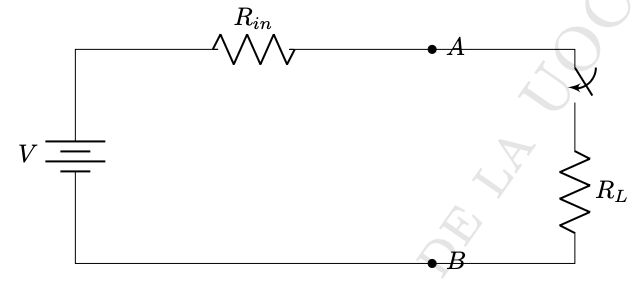
\includegraphics[width=10cm]{imagenes/enunciados/2_enunciado.png}
			\caption{Circuito de la Cuestión 2.}
		\end{figure} 

		Donde:

		\begin{enumerate}
			\item $V=230 \; V$
			\item $R_{in} = 2 \; \Omega$ representa la resistencia interna de los cables de alimentación debida a su resistividad.
			\item $L_{in} = 200 \; m$ es la longitud total del cable de alimentación que llega al enchufe (la longitud ya incluye el cable de ida y el de vuelta).
			\item $R_L = 20 \; \Omega$ representa el ventilador.
		\end{enumerate}

		Se conecta el ventilador al enchufe sin cerrar todavía el interruptor. Considerad que la resistividad del cobre tiene un valor $p=1,68 \cdot 10^{-8} \; \Omega \cdot \text{m}$.

		{ \color{blue} 
			\textbf{NOTA:} Todas las fórmulas de esta cuestión han sido tomadas del libro \textit{Circuitos eléctricos}.
		}

		\begin{enumerate}[label=\alph*)] 
			\item ¿Cuál es el valor de la tensión entre los puntos $A$ y $B$ antes de cerrar el interruptor para encender el ventilador?

				{ \color{blue} 
					Antes de cerrar el interruptor, el circuito se encuentra abierto. Puesto que no existe un camino cerrado, no se puede producir la circulación de electrones y, en consecuencia, la intensidad de corriente es nula ($I = 0 \text{ A}$). 

					Dado que no circula intensidad, la caída de tensión en la resistencia interna de los cables $R_{in}$ es de cero voltios, como podemos comprobar aislando la tensión a partir de la ley de Ohm en su ecuación (8): 
					$$V_{R_{in}} = I \cdot R_{in} = 0 \cdot 2 = 0 \text{ V}$$

					Por lo tanto, al no haber ninguna pérdida de tensión a lo largo de los cables, la diferencia de potencial entre los puntos $A$ y $B$ es exactamente igual a la tensión que proporciona la fuente principal:
						$$\boxed{V_{AB} = V = 230 \text{ V}}$$
				}

			\item ¿Cuál es el valor de la tensión entre los puntos $A$ y $B$ después de cerrar el interruptor para encender el ventilador?

				{ \color{blue} 
					Al cerrar el interruptor, establecemos un camino cerrado y se genera una corriente a través de los componentes. La resistencia interna de los cables ($R_{in}$) y la resistencia del ventilador ($R_L$) se encuentran asociadas en serie, pues circula la misma intensidad a través de ellas. Según indica la ecuación (14) del libro, la resistencia equivalente del circuito será la suma de ambas:
					$$R_{eq} = R_{in} + R_L = 2 \; \Omega + 20 \; \Omega = 22 \; \Omega$$

					Con este valor, aplicamos la ecuación (5) de la ley de Ohm para encontrar la corriente total del circuito:
					$$I = \frac{V}{R_{eq}} = \frac{230 \text{ V}}{22 \; \Omega} \approx 10,4545 \text{ A}$$

					La tensión entre los puntos $A$ y $B$ es justamente la caída de tensión en el ventilador $R_L$. Aplicando nuevamente la ley de Ohm (ecuación 8) sobre esta resistencia:
					$$\boxed{V_{AB} = I \cdot R_L = 10,4545 \text{ A} \cdot 20 \; \Omega \approx 209,09 \text{ V}}$$

					*(Nota: Este mismo resultado se obtiene aplicando directamente la ecuación (47) del divisor de tensión: $V_{AB} = V \cdot \frac{R_L}{R_{in} + R_L} = 230 \cdot \frac{20}{22} \approx 209,09 \text{ V}$).*
				}

			\vspace{0.5cm}

			\item Determinar la sección de los cables de alimentación.

				{ \color{blue} 
					Para calcular la sección, utilizamos la ecuación (2) que define la resistencia de un elemento en función de sus características geométricas y su material:
					$$R = \rho \frac{L}{S}$$

					Donde $R$ es la resistencia del cable ($R_{in} = 2 \; \Omega$), $\rho$ es la resistividad del cobre ($1,68 \cdot 10^{-8} \; \Omega \cdot \text{m}$), $L$ es la longitud total del conductor ($200 \text{ m}$) y $S$ es la sección que buscamos.

					Despejando la sección $S$ de la fórmula anterior, tenemos:
					$$S = \rho \frac{L}{R_{in}} = 1,68 \cdot 10^{-8} \; \Omega \cdot \text{m} \cdot \frac{200 \text{ m}}{2 \; \Omega} = 1,68 \cdot 10^{-6} \text{ m}^2$$

					Si transformamos este resultado a milímetros cuadrados (una unidad de medida más común para la superficie en electrónica), obtenemos:
					$$\boxed{S = 1,68 \text{ mm}^2}$$
				}

			\item Si el ventilador necesitara una tensión mínima de $215 \; \text{V}$ para funcionar, ¿qué solución propondríais?

				{ \color{blue} 
					En el apartado b) hemos determinado que la tensión real que llega a los terminales $A$ y $B$ del ventilador es de aproximadamente $209,09 \text{ V}$. Si este necesita $215 \text{ V}$ para funcionar, existe una pérdida excesiva de tensión en el trayecto.

					Para conseguir que la tensión $V_{AB}$ aumente, es necesario reducir la caída de tensión en los cables de alimentación, lo cual requiere disminuir de alguna manera la resistencia interna $R_{in}$ del tramo.

					Basándonos en la ecuación (2) y en las propiedades de los materiales, sabemos que la resistencia es menor cuanto menor sea su longitud y mayor su sección. Puesto que el material de la instalación es cobre y la distancia física entre la fuente y el enchufe (la longitud $L$) está normalmente fija por la construcción, la solución técnica ideal es \textbf{aumentar la sección transversal $S$ de los cables de alimentación}. Sustituyendo el cableado actual por unos cables de cobre más gruesos (con una sección de conductor mayor), lograremos bajar el valor de $R_{in}$ y, en consecuencia, minimizar la caída de voltaje en ellos logrando superar el umbral de los $215 \text{ V}$ en el ventilador.
				}
		\end{enumerate}
	\end{problem}

	% --- Exercise 3 ---
	\begin{problem}[Cuestión 3]
		Tenemos el circuito de la figura siguiente:

		\begin{figure}[H]
			\centering
			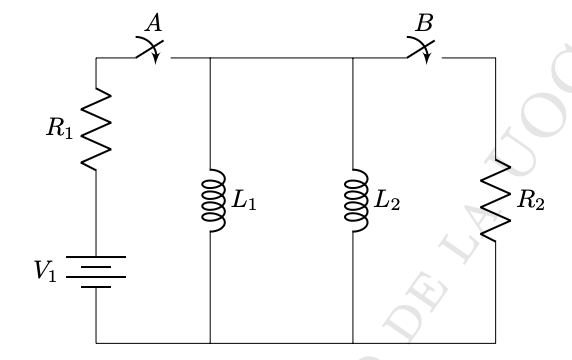
\includegraphics[width=10cm]{imagenes/enunciados/3_enunciado.png}
			\caption{Circuito de la Cuestión 3.}
		\end{figure} 

		Donde:

		\begin{enumerate}
			\item $V_1=30 \; \text{V}$
			\item $R_1 = 3 \; \Omega$ 
			\item $L_1 = L_2 = 6 \; \text{H}$
			\item $R_2 = 1 \; \Omega$ representa el ventilador.
		\end{enumerate}

		Inicialmente, los dos interruptores (A y B) se encuentran abiertos. En el instante $t=0$, el interruptor A se cierra (el interruptor B continúa abierto). En el instante $t=1 \; \text{s}$, el interruptor A se abre de nuevo y el interruptor B se cierra.

		{ \color{blue} 
			\textbf{NOTA:} Todas las fórmulas de esta cuestión han sido tomadas del libro \textit{Circuitos RLC}.
		}

		\begin{enumerate}[label=\alph*)] 
			\item Determinar la bobina equivalente a las dos bobinas $L_1$ y $L_2$.

				{ \color{blue} 
					Para determinar la bobina equivalente de $L_1$ y $L_2$, observamos en el circuito que ambas están conectadas en paralelo. La inductancia equivalente a un conjunto de bobinas conectadas en paralelo se obtiene calculando el inverso de la suma de los inversos de los coeficientes de las bobinas originales, tal como establece la ecuación (84) del libro:
					$$\frac{1}{L_{eq}} = \frac{1}{L_1} + \frac{1}{L_2}$$

					Para el caso de dos bobinas, podemos utilizar la expresión simplificada equivalente al producto dividido por la suma:
					$$L_{eq} = \frac{L_1 \cdot L_2}{L_1 + L_2}$$

					Sustituyendo los valores dados:
					$$\boxed{L_{eq} = \frac{6 \text{ H} \cdot 6 \text{ H}}{6 \text{ H} + 6 \text{ H}} = \frac{36}{12} = 3 \text{ H}}$$
				}

			\item Deteminar la expresión de la corriente que circula por la resistencia $R_1$ entre los instantes $t=0$ y $t=1$ s.

				{ \color{blue} 
					Al cerrar el interruptor A (y con B abierto), la fuente $V_1$, la resistencia $R_1$ y la bobina equivalente $L_{eq}$ quedan conectadas en serie, formando un circuito RL en proceso de carga.

					La expresión de la intensidad para un circuito RL en carga viene dada por la ecuación (60):
					$$i(t) = \frac{V_1}{R_1} \left(1 - e^{-\frac{R_1}{L_{eq}}t}\right)$$

					Donde la constante de tiempo $\tau$ se define en la ecuación (66) como $\tau = \frac{L_{eq}}{R_1}$. 

					Sustituyendo nuestros valores ($V_1 = 30 \text{ V}$, $R_1 = 3 \; \Omega$ y $L_{eq} = 3 \text{ H}$), obtenemos:
					$$\boxed{i(t) = \frac{30}{3} \left(1 - e^{-\frac{3}{3}t}\right) = 10 \left(1 - e^{-t}\right) \text{ A}}$$
				}

			\item Determinar la corriente que circula por la resistencia en el instante $t=1$ s (justo antes del cambio de los interruptores).

				{ \color{blue} 
					Para hallar esta corriente, basta con evaluar la expresión matemática obtenida en el apartado anterior en el instante $t = 1 \text{ s}$:
					$$i(1) = 10 \left(1 - e^{-1}\right) \text{ A}$$

					Dado que el valor de $e^{-1} \approx 0,3678$:
					$$\boxed{i(1) \approx 10 \cdot (1 - 0,3678) = 10 \cdot 0,6322 = 6,322 \text{ A}}$$
				}

			\item Calcular el valor de la tensión que cae sobre las bobinas $L_1$ y $L_2$ en el instante $t = 1$ s (justo antes del cambio de los interruptores).

				{ \color{blue} 
					Dado que $L_1$ y $L_2$ se encuentran en paralelo, la tensión que cae sobre cada una de ellas es la misma, y corresponde a la tensión de la bobina equivalente $L_{eq}$. Durante el proceso de carga de un circuito RL, la evolución de la tensión en la bobina está dictada por la ecuación (62):
					$$v_L(t) = V_1 \cdot e^{-\frac{R_1}{L_{eq}}t}$$

					Evaluando en el instante $t=1 \text{ s}$ con los valores de nuestro circuito:
					$$\boxed{v_L(1) = 30 \cdot e^{-\frac{3}{3}\cdot 1} = 30 \cdot e^{-1} \approx 30 \cdot 0,3678 = 11,034 \text{ V}}$$
				}

			\item Determinar el valor de la corriente que circula por la resistencia $R_2$ justo después del cambio de los interruptores, y transcurrido un tiempo muy largo.

				{ \color{blue} 
					En el instante $t=1 \text{ s}$, el interruptor A se abre, desconectando la fuente $V_1$, y el interruptor B se cierra. A partir de este momento, la bobina equivalente $L_{eq}$ comienza un proceso de descarga a través de la resistencia $R_2$.

					\textbf{Justo después del cambio:}
					Una propiedad fundamental de las bobinas es que la intensidad de la corriente que circula por ellas no puede presentar saltos bruscos. Por consiguiente, la corriente que circulará por la nueva malla formada por $L_{eq}$ y $R_2$ justo después del cambio será exactamente la misma que circulaba por la bobina justo antes del cambio. Es decir, $\boxed{i(1^+) = i(1^-) \approx 6,322 \text{ A}}$.

					\textbf{Transcurrido un tiempo muy largo:}
					Al dejar al circuito evolucionar sin ninguna fuente de alimentación externa, el sistema entra en la fase de descarga descrita por la ecuación (69). Transcurrido un tiempo suficientemente grande (al alcanzar el régimen permanente), la energía acumulada en la bobina se habrá disipado por completo en forma de calor en la resistencia $R_2$, y la intensidad que circulará por el circuito será de $\boxed{0 \text{ A}}$.
				}
		\end{enumerate}
	\end{problem}

	% --- Exercise 4 ---
	\begin{problem}[Cuestión 4]
		Tenemos el circuito de la figura 4:

		\begin{figure}[H]
			\centering
			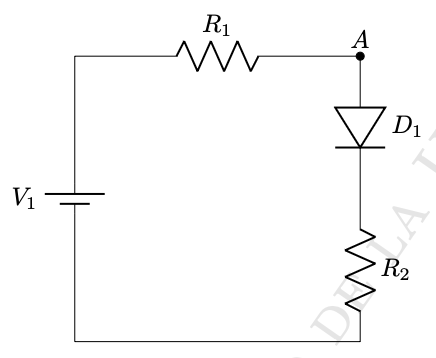
\includegraphics[width=10cm]{imagenes/enunciados/4_enunciado.png}
			\caption{Circuito de la Cuestión 4.}
		\end{figure} 

		Datos del circuito:

		\begin{enumerate}
			\item $V_1=15 \; V$
			\item $R_1 = 220 \; \Omega; R_2 = 100 \; \Omega$ 
			\item $D_1 \text{(Silicio)}: \text{Tensión umbral } V_{\gamma} = 0,7 \; V$
		\end{enumerate}

		Se pide:

		{ \color{blue} 
			\textbf{NOTA:} Todas las fórmulas de esta cuestión han sido tomadas del libro \textit{Circuitos eléctricos}.
		}

		\begin{enumerate}[label=\alph*)] 
			\item Si el diodo se encuentra en conducción (ON), ¿cuál es la tensión entre sus extremos?

				{ \color{blue} 
					Basándonos en el modelo equivalente del diodo para su estado de conducción (ON), la tensión entre sus extremos queda fijada en su tensión umbral $V_{\gamma}$. Por lo tanto, la tensión que cae sobre el diodo es:
					$$\boxed{V_{D1} = V_{\gamma} = 0,7 \text{ V}}$$
				}

			\item Calcular la intensidad de corriente que circula por la resistencia $R_1$.

				{ \color{blue} 
					Dado que todos los componentes están conectados formando un único camino cerrado, conforman una asociación en serie, por lo que la corriente $I$ que circula por la resistencia $R_1$ es exactamente la misma que circula por todo el circuito. 

					Para calcularla, aplicamos la segunda ley de Kirchhoff (ley de las tensiones), que establece que la suma algebraica de las tensiones en una malla es cero:
					$$V_1 - V_{R1} - V_{D1} - V_{R2} = 0$$

					Aplicando la ley de Ohm expresada en la ecuación (4) del libro, sabemos que la caída de tensión en una resistencia es $V = I \cdot R$. Sustituyendo esto en nuestra ecuación y reordenando los términos:
					$$V_1 - V_{D1} = I \cdot R_1 + I \cdot R_2 = I \cdot (R_1 + R_2)$$

					Donde $(R_1 + R_2)$ se corresponde con la resistencia equivalente de una asociación en serie descrita por la ecuación (14). Despejando la intensidad $I$:
					$$I = \frac{V_1 - V_{D1}}{R_1 + R_2}$$

					Sustituyendo los valores numéricos proporcionados:
					$$I = \frac{15 \text{ V} - 0,7 \text{ V}}{220 \; \Omega + 100 \; \Omega} = \frac{14,3 \text{ V}}{320 \; \Omega} \approx 0,04469 \text{ A}$$

					Expresando el resultado final en miliamperios:
					$$\boxed{I = 44,69 \text{ mA}}$$
				}

			\item Determinar si la hipótesis de conducción (ON) era correcta.

				{ \color{blue} 
					Para que un diodo se encuentre operando en la zona de conducción (estado ON), se le debe aplicar una tensión positiva superior a su umbral, de modo que deje pasar la corriente (es decir, que la corriente a su través presente un valor positivo fluyendo de ánodo a cátodo). 

					Al realizar el análisis bajo la hipótesis de conducción, hemos obtenido una corriente $I \approx 44,69 \text{ mA}$. Puesto que el valor resultante es positivo ($I > 0$), se confirma que la corriente circula en el sentido permitido por el componente. Por lo tanto, la hipótesis inicial de que el diodo se encontraba en conducción (ON) \textbf{era correcta}.
				}
		\end{enumerate}
	\end{problem}

	% -- Exercise 5 ---
	\begin{problem}[Cuestión 5]
		Tenemos el circuito de la figura 5:

		\begin{figure}[H]
			\centering
			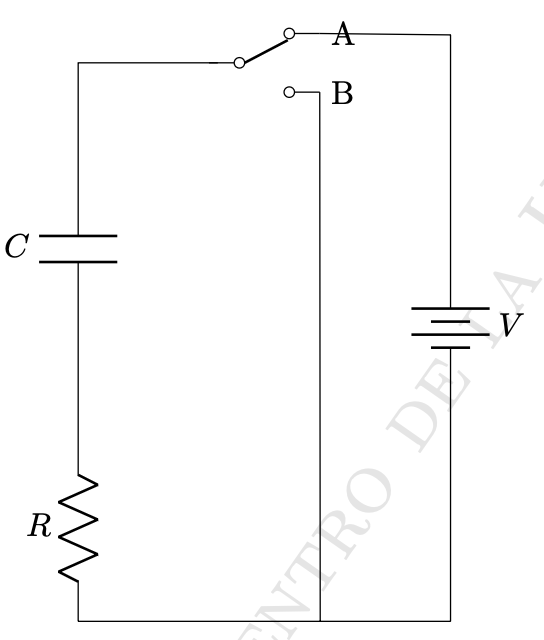
\includegraphics[width=10cm]{imagenes/enunciados/5_enunciado.png}
			\caption{Circuito de la Cuestión 5.}
		\end{figure} 

		Inicialmente, el conmutador se encuentra en la posición A y el circuito se encuentra en régimen permanente. En el instante de tiempo $t=0$, el conmutador cambia a la posición B.

		Determinar si las siguientes afirmaciones son \textbf{CIERTAS} o \textbf{FALSAS}, y justificad la respuesta.

		{ \color{blue} 
			\textbf{NOTA:} Todas las fórmulas de esta cuestión han sido tomadas del libro \textit{Circuitos RLC}.
		}

		\begin{enumerate}[label=\alph*)] 
			\item En el régimen permanente antes de $t = 0$, circula una corriente constante máxima por la resistencia $R$.

				{ \color{blue} 
					\textbf{FALSA}. Si trabajamos en corriente continua, el condensador se comporta como un circuito abierto una vez llega a su régimen permanente. En esta situación transitoria final, el condensador se encuentra totalmente cargado almacenando una tensión igual a la de la fuente $V$, y al actuar como un camino abierto, la corriente que circula por la resistencia $R$ y por el resto del circuito es nula ($I = 0 \text{ A}$).
				}

			\vspace{0.5cm}

			\item En el instante $t=0$, al cambiar el conmutador a la posición B, la tensión en los extremos del condensador pasa a ser exactamente de 0 V.

				{ \color{blue} 
					\textbf{FALSA}. Una propiedad fundamental matemática y física que define el comportamiento del condensador es que la tensión entre sus dos extremos no puede variar bruscamente, ya que esto requeriría una corriente infinita. Puesto que antes de accionar el conmutador ($t = 0^-$) el condensador estaba cargado con la tensión $V$, en el instante justo después del cambio ($t = 0^+$) mantendrá exactamente esa misma tensión de $V$ voltios. Comienza su proceso de descarga a partir de ese valor inicial.
				}

			\vspace{0.5cm}

			\item Después de cambiar el conmutador, el condensador se descargará manteniendo una corriente de descarga constante en el tiempo.

				{ \color{blue} 
					\textbf{FALSA}. Durante el proceso de descarga, la intensidad que circula por el circuito no es constante, sino que sigue una forma exponencial a medida que transcurre el tiempo. Al desconectar la fuente (posición B), el condensador se descarga a través de la resistencia $R$. La intensidad de esta corriente de descarga sigue un perfil exponencial decreciente regido por la ecuación (34) del libro: 
					$$i(t) = -\frac{V}{R} e^{-\frac{t}{RC}}$$ 

					Y la evolución de la tensión en el condensador decae según la ecuación (36):
					$$v_C(t) = V e^{-\frac{t}{RC}}$$
					donde $RC$ equivale a la constante de tiempo $\tau$. Por lo tanto, la corriente de descarga va decreciendo y tiende a anularse conforme el circuito alcanza su estado de reposo.
				}
		\end{enumerate}
	\end{problem}

		% -- Exercise 6 ---
	\begin{problem}[Cuestión 6]
		En este ejercicio comprobaremos el funcionamiento de un circuito complejo con diodos, realizando una simulación interactiva del circuito.

		Considerad el circuito de la figura 6.

		\begin{figure}[H]
			\centering
			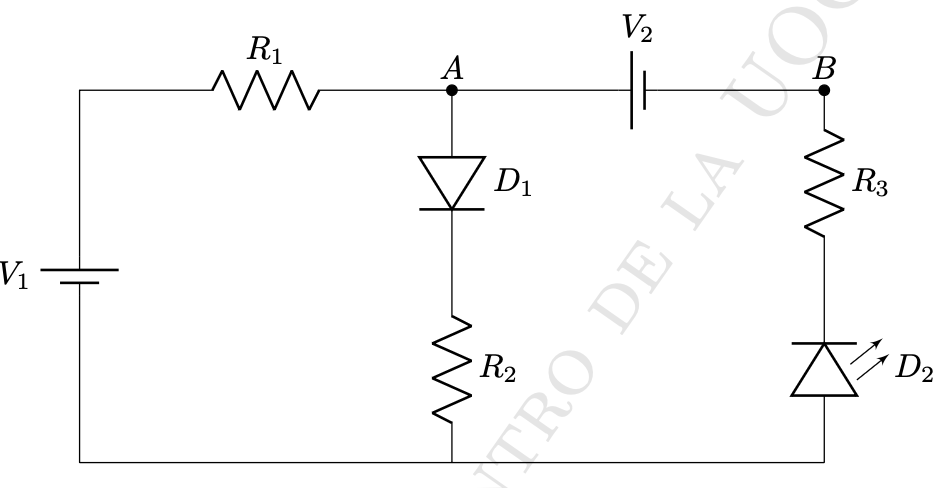
\includegraphics[width=11cm]{imagenes/enunciados/6_enunciado.png}
			\caption{Figura 6: Circuito de la Cuestión 6.}
		\end{figure} 

		Datos del circuito:

		\begin{enumerate}
			\item $V_1=15 \; \text{V}$
			\item $V_2 = 5$ 
			\item $R_1 = 220 \; \Omega, R_2 = 100 \; \Omega, R_3 = 470 \; \Omega$
			\item $D_1 \text{(Silicio): Tensión umbral } V_{\gamma 1} = 0,7 \; \text{V}$
			\item $D_2 \text{(LED): Tensión umbral } V_{\gamma 2} = 2,0 \; \text{V}$
		\end{enumerate}

		Utilizaremos el simulador de circuitos en línea \textbf{Falstad} (https://www.falstad.com/circuit/), que es gratuito, funciona directamente en el navegador web y permite visualizar el flujo de corriente de manera muy intuitiva. Asimismo, más allá de las herramientas de medida habituales (voltímetros, amperímetros, etc.), permite medir directamente algunos parámetros "pinchando" el circuito mediante \textit{test points}.

		\textbf{Simulación}

		\begin{enumerate}[label=\alph*)] 
			\item \textbf{Análisis del estado inicial} $(V_1 = 15 \; \text{V})$

				Añadid voltímetros (\textbf{Draw $\rightarrow$ Outputs and Labels $\rightarrow$ Add Voltmeter}) conectados entre los nodos A y B y al nodo de referencia (masa inferior). También podéis utilizar (\textbf{Draw} $\rightarrow$ \textbf{Outputs and Labels} $\rightarrow$ \textbf{Add Test Point}) que no necesita conexión al nodo inferior.

				\begin{itemize}
					\item Comprobad visualmente qué diodo está conduciendo (el simulador muestra puntos amarillos moviéndose para indicar la corriente, si conduce).
					\item Haced una captura de pantalla donde se vean claramente las tensiones medidas en los nodos A y B. ¿Coinciden aproximadamente con los $5,168 \; \text{V}$ y $0,168 \; \text{V}$ teóricos?
				\end{itemize}

				{ \color{blue} 
					Al contrastar estos cálculos teóricos con la simulación en Falstad, se observa una ligera discrepancia. El simulador muestra unos valores de $V_A = 4,747 \text{ V}$ y $V_B = -0,253 \text{ V}$. Esta diferencia se debe a que el cálculo teórico asume un modelo ideal simplificado con una caída de tensión fija de $0,7 \text{ V}$ para $D_1$, mientras que Falstad utiliza un modelo de diodo más complejo basado en la ecuación de Shockley con parámetros reales de resistencia interna. No obstante, los valores simulados confirman la premisa teórica principal, la cual es que la tensión resultante en el nodo B es insuficiente para superar la barrera de $2,0 \text{ V}$ del LED ($D_2$).

					\begin{figure}[H]
						\centering
						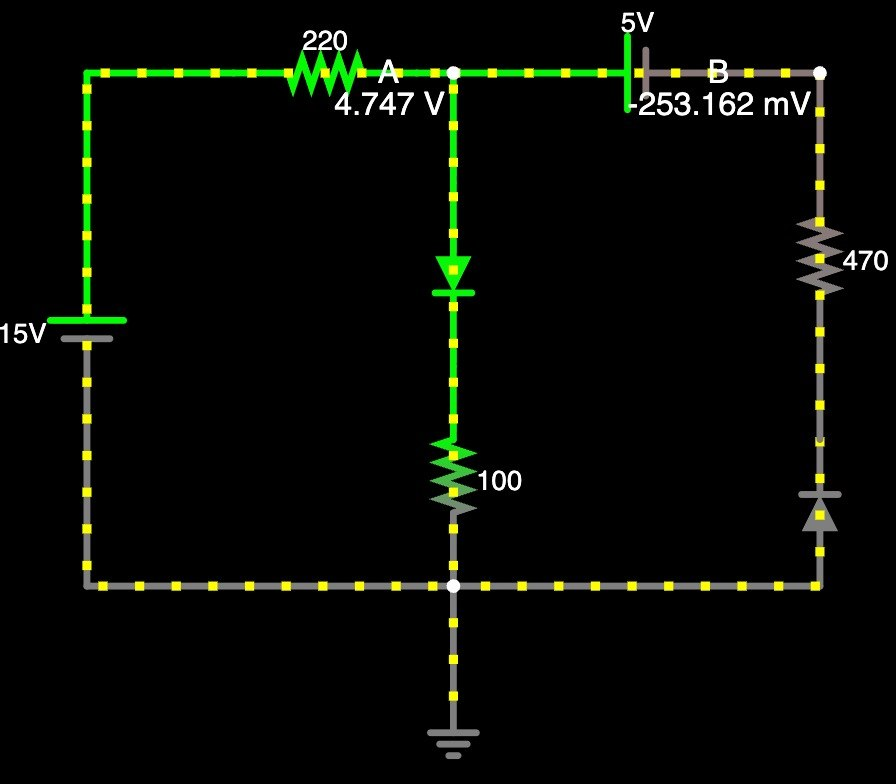
\includegraphics[width=10cm]{imagenes/6a.jpg}
						\caption{Análisis del estado inicial}
					\end{figure} 
				}

			\item \textbf{Corriente por $R_1$}

				Podéis ver la corriente pasando el ratón por encima de la resistencia $R_1$ o bien añadiendo un amperíemtro en serie (\textbf{Draw} $\rightarrow$ \textbf{Outputs and Labels} $\rightarrow$ \textbf{Add Ammeter}).

				\begin{itemize}
					\item Haced una captura de pantalla donde se vea claramente el valor de la corriente mostrado por el simulador. ¿Coincide con los 44,7 mA calculados teóricamente?
				\end{itemize}

				{ \color{blue} 
					Tal y como se observa en la captura de pantalla, al consultar los datos del componente $R_1$ en el simulador, este indica una corriente de $46,605\text{ mA}$. Este valor coincide de forma aproximada con los $44,7\text{ mA}$ calculados teóricamente. La ligera desviación de unos $1,9\text{ mA}$ es coherente con la discrepancia de tensiones observada en el nodo A durante el apartado anterior. Dado que el cálculo teórico asume una caída ideal y fija de $0,7\text{ V}$ en el diodo $D_1$, la corriente teórica resulta ser ligeramente inferior a la obtenida en Falstad, cuyo modelo físico calcula una caída de tensión en el diodo algo menor, permitiendo así el paso de una corriente levemente mayor en la simulación.

					\begin{figure}[H]
						\centering
						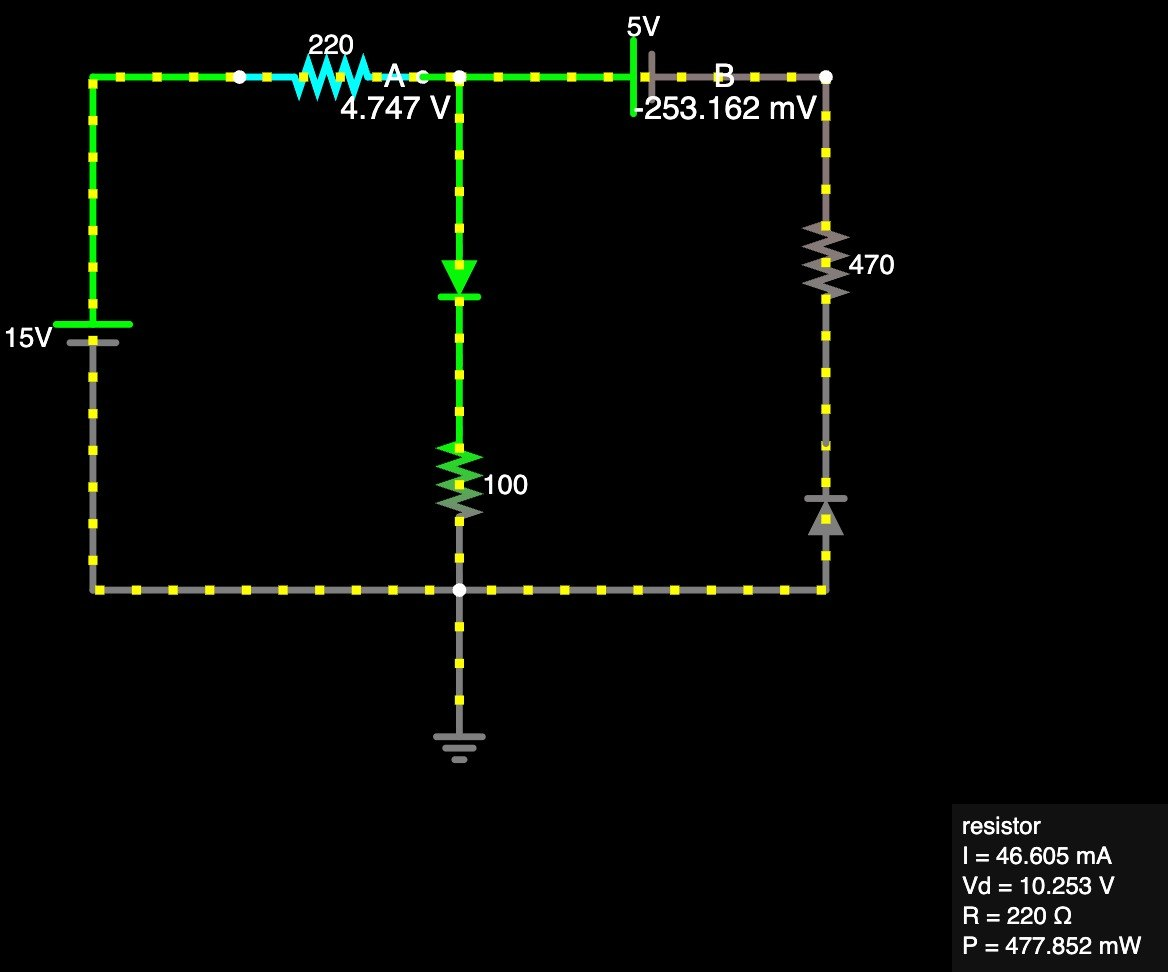
\includegraphics[width=10cm]{imagenes/6b.jpg}
						\caption{Corriente por $R_1$}
					\end{figure}
				}

			\item \textbf{Comprobación del umbral de conducción del diodo $D_2$} .

				Para comprobar el tercer apartado, haced clic derecho sobre la fuente $V_1$ y seleccionar \textbf{Sliders}. Esto hará aparecer una barra deslizante a la derecha de la pantalla para variar la tensión de la fuente en tiempo real.

				\begin{itemize}
					\item Reducid poco a poco el valor de $V_1$ hasta que observéis que el LED comienza a conducir (comienza a pasar corriente de abajo a arriba).
					\item Buscad el valor exacto de $V_1$ donde la tensión en el nodo B baja justo por debajo de $-2$ V. ¿Qué valor de $V_1$ muestra el deslizador en este punto de transición? ¿Es próximo a los 8,06 calculados?
				\end{itemize}

				{ \color{blue} 
					Al reducir el valor de $V_1$ con el deslizador, observamos que en torno a los $8,4\text{ V}$ la tensión en el nodo B desciende por debajo de los $-2,0\text{ V}$ ($V_B = -2,062\text{ V}$). En este punto exacto se supera la tensión umbral de $2,0\text{ V}$ del diodo $D_2$ y la corriente comienza a pasar de abajo a arriba. 

					El valor obtenido de $\approx 8,4\text{ V}$ es muy cercano a los $8,06\text{ V}$ calculados teóricamente. La pequeña discrepancia es esperable debido a que el modelo físico que emplea Falstad para el diodo $D_1$ es dinámico y no asume una caída fija e ideal de $0,7\text{ V}$ en todo el rango de corrientes.

					\begin{figure}[H]
						\centering
						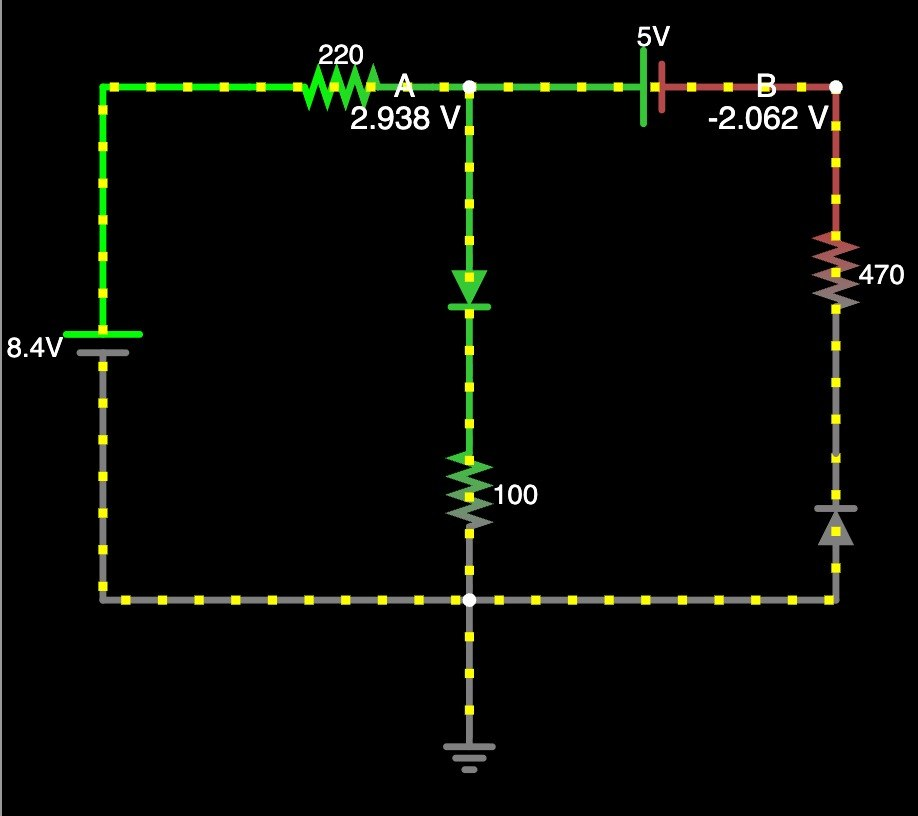
\includegraphics[width=10cm]{imagenes/6c.jpg}
						\caption{Corriente por $D_2$}
					\end{figure}
				}
		\end{enumerate}
	\end{problem}

	% --- Problem ---
	\begin{problem}[Problema]
		Tenemos el circuito de la figura 7:

		\begin{figure}[H]
			\centering
			
\includegraphics[width=11cm]{problema_enunciado.png}
			\caption{Figura 7: Circuito con mallas A, B y C.}
		\end{figure} 

		Los valores de los elementos del circuito son los siguientes: $V_1 = 12 \; \text{V}, V_2 = 10 \; \text{V}, R_1 = 2 \; \Omega, R_2 = 4 \; \Omega, R_3 = 2 \; \Omega, R_4 = 4 \; \Omega$ y $R_5 = 1 \; \Omega$.

		Se pide lo siguiente:

		\begin{enumerate}[label=\alph*)] 
			\item Calcular las corrientes de malla $I_A$, $I_B$ y $I_C$ (considerándolas en sentido horario).

				{ \color{blue} 
					Para calcular las corrientes de malla, aplicamos la segunda ley de Kirchhoff (ley de las tensiones) a cada una de las mallas, recorriéndolas en el sentido horario propuesto,. Siguiendo el método sistemático de las corrientes de malla,, sumamos las caídas de tensión en las resistencias y las fuentes de voltaje:

					\textbf{Malla A:}
					$$-V_1 + I_A R_1 + (I_A - I_B) R_2 = 0$$
					$$-12 + 2 I_A + 4 (I_A - I_B) = 0 \implies 6 I_A - 4 I_B = 12 \implies 3 I_A - 2 I_B = 6$$

					\textbf{Malla B:}
					$$(I_B - I_A) R_2 + I_B R_3 + (I_B - I_C) R_4 = 0$$
					$$4 (I_B - I_A) + 2 I_B + 4 (I_B - I_C) = 0 \implies -4 I_A + 10 I_B - 4 I_C = 0 \implies -2 I_A + 5 I_B - 2 I_C = 0$$

					\textbf{Malla C:}
					$$(I_C - I_B) R_4 + V_2 + I_C R_5 = 0$$
					Al recorrer la malla C en sentido horario, pasamos por la fuente $V_2$ entrando por su terminal positivo, lo que representa una subida o caída de tensión positiva en nuestra ecuación de malla,.
					$$4 (I_C - I_B) + 10 + 1 I_C = 0 \implies -4 I_B + 5 I_C = -10$$

					Tenemos un sistema de tres ecuaciones. Despejando $I_C$ de la tercera ecuación obtenemos $I_C = 0,8 I_B - 2$. Sustituyendo esto en la segunda:
					$$-2 I_A + 5 I_B - 2(0,8 I_B - 2) = 0 \implies -2 I_A + 3,4 I_B + 4 = 0 \implies I_A = 1,7 I_B + 2$$

					Sustituyendo $I_A$ en la primera ecuación:
					$$3(1,7 I_B + 2) - 2 I_B = 6 \implies 5,1 I_B + 6 - 2 I_B = 6 \implies 3,1 I_B = 0 \implies I_B = 0 \text{ A}$$

					Con $I_B = 0 \text{ A}$, calculamos el resto:
					$$I_A = 1,7(0) + 2 = 2 \text{ A}$$
					$$I_C = 0,8(0) - 2 = -2 \text{ A}$$

					Por lo tanto, las corrientes de malla son: $\boxed{I_A = 2 \text{ A}}$, $\boxed{I_B = 0 \text{ A}}$ e $\boxed{I_C = -2 \text{ A}}$.
				}

			\vspace{0.5cm}

			\item Determinar el valor y el sentido de la corriente que circula por cada una de las resistencias ($R_1,R_2,R_3,R_4,R_5$).

				{ \color{blue} 
					La corriente real en cada resistencia se determina superponiendo las corrientes de malla que la atraviesan,. Un valor negativo en el resultado indica que la corriente fluye en sentido contrario al supuesto inicialmente.
					\begin{itemize}
						\item \textbf{$R_1$:} Solo la atraviesa $I_A$. Su valor es $I_{R1} = I_A = 2 \text{ A}$. El sentido es de izquierda a derecha.
						\item \textbf{$R_2$:} Compartida por las mallas A y B. Su valor hacia abajo es $I_{R2} = I_A - I_B = 2 - 0 = 2 \text{ A}$. El sentido es hacia abajo.
						\item \textbf{$R_3$:} Solo la atraviesa $I_B$. Su valor es $I_{R3} = I_B = 0 \text{ A}$. No circula corriente por ella.
						\item \textbf{$R_4$:} Compartida por las mallas B y C. Su valor hacia abajo es $I_{R4} = I_B - I_C = 0 - (-2) = 2 \text{ A}$. El sentido es hacia abajo.
						\item \textbf{$R_5$:} Solo la atraviesa $I_C$. Su valor respecto al sentido horario es $I_{R5} = I_C = -2 \text{ A}$. Al ser negativo, la corriente real fluye en sentido contrario. Su valor es $2 \text{ A}$ y el sentido es hacia arriba.
					\end{itemize}
				}

			\item Calcular la caída de tensión en la resistencia $R_2$.

				{ \color{blue} 
					Para calcular la caída de tensión en $R_2$, aplicamos directamente la ley de Ohm, definida por la ecuación (4) del libro.
					$$V_{R2} = I_{R2} \cdot R_2$$
					Sustituyendo los valores obtenidos en el apartado anterior ($I_{R2} = 2 \text{ A}$ y $R_2 = 4 \;\Omega$):
					$$\boxed{V_{R2} = 2 \text{ A} \cdot 4 \;\Omega = 8 \text{ V}}$$
				}

			\item Calcular la tensión equivalente de Thévenin entre los terminales $E$ y $F$ ($V_{Th}$).

				{ \color{blue} 
					El teorema de Thévenin establece que la tensión equivalente de Thévenin ($V_{Th}$) es la tensión existente entre los terminales de interés cuando estos se encuentran en circuito abierto. Dado que en el esquema proporcionado no hay ninguna carga conectada entre E y F, las corrientes del circuito son exactamente las calculadas en el apartado a).

					Los terminales E y F se corresponden a los nodos superior e inferior de la rama más a la derecha. Podemos calcular esta diferencia de potencial observando la rama de $R_4$ o bien la rama derecha ($V_2$ y $R_5$):

					A través de $R_4$:
					$$V_{Th} = V_E - V_F = V_{R4} = I_{R4} \cdot R_4 = 2 \text{ A} \cdot 4 \;\Omega = 8 \text{ V}$$

					A través de la rama derecha (recorriendo desde F hasta E):
					$$V_{Th} = V_E - V_F = V_2 + I_{R5 (\text{hacia abajo})} \cdot R_5 = 10 \text{ V} + (-2 \text{ A}) \cdot 1 \;\Omega = 8 \text{ V}$$

					Por lo tanto, la tensión equivalente de Thévenin es $\boxed{V_{Th} = 8 \text{ V}}$.
				}

			\vspace{0.5cm}

			\item Calcular la resistencia equivalente de Thévenin entre los terminales $E$ y $F$ ($R_{Th}$).

				{ \color{blue} 
					La resistencia equivalente de Thévenin ($R_{Th}$) es la resistencia que se "ve" desde los terminales E y F tras desactivar todas las fuentes independientes (las fuentes de tensión se sustituyen por cortocircuitos),.

					Al sustituir $V_1$ y $V_2$ por un cortocircuito, evaluamos las asociaciones resultantes mirando desde E y F hacia el interior del circuito:

					Al cortocircuitar $V_1$, $R_1$ queda conectada en paralelo con $R_2$. Según la ecuación (26) de resistencias en paralelo:
					$$R_{12} = \frac{R_1 \cdot R_2}{R_1 + R_2} = \frac{2 \cdot 4}{2 + 4} = \frac{8}{6} = \frac{4}{3} \;\Omega$$

					Esta resistencia equivalente $R_{12}$ queda en serie con $R_3$. Aplicando la ecuación (14):
					$$R_{123} = R_{12} + R_3 = \frac{4}{3} + 2 = \frac{10}{3} \;\Omega$$

					Este conjunto $R_{123}$ queda en paralelo con $R_4$:
					$$R_{1234} = \frac{R_{123} \cdot R_4}{R_{123} + R_4} = \frac{\frac{10}{3} \cdot 4}{\frac{10}{3} + 4} = \frac{40/3}{22/3} = \frac{40}{22} = \frac{20}{11} \;\Omega$$

					Finalmente, al estar la fuente $V_2$ cortocircuitada, la resistencia $R_5$ queda conectada directamente entre los terminales E y F, situándose en paralelo con el resto del circuito equivalente ($R_{1234}$):
					$$R_{Th} = \frac{R_{1234} \cdot R_5}{R_{1234} + R_5} = \frac{\frac{20}{11} \cdot 1}{\frac{20}{11} + 1} = \frac{20/11}{31/11} = \frac{20}{31} \;\Omega \approx 0,645 \;\Omega$$

					La resistencia equivalente de Thévenin es $\boxed{R_{Th} = \frac{20}{31} \;\Omega}$.
				}
		\end{enumerate}
	\end{problem}
\end{document}
